\subsection{Experiments}

Below are the conducted experiments to answer the proposed research questions.
% \begin{table*}[t!]
\centering
\scriptsize
\setlength{\tabcolsep}{3.5pt}
\renewcommand{\arraystretch}{1.1}
\scalebox{0.85}{
\begin{tabular}{l l*{8}{c}}
\toprule
\multirow{2}{*}{\textbf{LLM Backbone}} & \multirow{2}{*}{\textbf{Method}} & \multicolumn{6}{c}{\textbf{Exact Match $\uparrow$}} & \multicolumn{1}{c}{\textbf{API / Acc. $\uparrow$}}\\
\cmidrule(lr){3-8}\cmidrule(lr){9-9}
 &  & AIME24 & AIME25 & GPQA & MMLU-Pro (Eco.) & MMLU-Pro (Eng.) & MMLU-Pro (Philo.) & ToolBench& \multicolumn{1}{c}{\textbf{Avg. $\uparrow$}}\\
\midrule

% ---------------- Claude 3.5 ----------------
\multirow{15}{*}{Claude 3.5}
 & Baseline   & \textemdash{} & \textemdash{} & 0.36 & 0.68 & 0.42 & 0.55 & 0.81/0.64 & 0.38 \\
 & History    & \textemdash{} & \textemdash{} & 0.37 & 0.70 & 0.43 & 0.55 & 0.81/0.63 & 0.38 \\
\cmidrule(lr){2-10}
 & ReAct      & \textemdash{} & \textemdash{} & 0.35 & 0.69 & 0.43 & 0.54 & 0.81/0.64 & 0.38 \\
 & Amem       & \textemdash{} & \textemdash{} & 0.34 & 0.69 & 0.43 & 0.53 & 0.82/0.63 & 0.37 \\
\cmidrule(lr){2-10}
 & SelfRAG    & \textemdash{} & \textemdash{} & 0.36 & 0.70 & 0.44 & 0.56 & 0.83/0.65 & 0.39 \\
 & MemOS      & \textemdash{} & \textemdash{} & 0.37 & 0.70 & 0.42 & 0.55 & 0.81/0.64 & 0.38 \\
 & Mem0       & \textemdash{} & \textemdash{} & 0.36 & 0.70 & 0.42 & 0.55 & 0.82/0.64 & 0.38 \\
 & LangMem    & \textemdash{} & \textemdash{} & \textbf{0.51} & \textbf{0.78} & 0.46 & 0.61 & 0.81/0.63 & \textbf{0.43} \\
\cmidrule(lr){2-10}
 & DC-RS      & \textemdash{} & \textemdash{} & 0.36 & 0.68 & 0.41 & 0.56 & 0.82/0.64 & 0.38 \\
 & AWM        & \textemdash{} & \textemdash{} & 0.33 & 0.67 & 0.42 & 0.53 & 0.81/0.63 & 0.37 \\
 & DC-Cu      & \textemdash{} & \textemdash{} & 0.33 & 0.65 & 0.39 & 0.54 & 0.82/0.63 & 0.36 \\
\cmidrule(lr){2-10}
 & ExpRecent  & \textemdash{} & \textemdash{} & 0.42 & 0.69 & 0.46 & 0.59 & 0.85/0.63 & 0.40 \\
 & ExpRAG     & \textemdash{} & \textemdash{} & 0.40 & 0.73 & \textbf{0.49} & 0.61 & 0.87/0.67 & 0.41 \\
 & ReMem      & \textemdash{} & \textemdash{} & 0.39 & 0.71 & 0.47 & \textbf{0.62} & \textbf{0.87/0.68} & 0.41 \\
\midrule

% ---------------- Claude 3.7 ----------------
\multirow{15}{*}{Claude 3.7 Sonnet}
 & Baseline            & 0.17 & 0.13 & 0.55 & 0.84 & 0.63 & 0.78 & 0.76/0.62 & 0.54 \\
 & History       & 0.13 & \textbf{0.23} & 0.56 & 0.85 & 0.64 & 0.78 & 0.76/0.61 & 0.55 \\
\cmidrule(lr){2-10}
 & ReAct                     & 0.17 & 0.10 & 0.57 & 0.84 & 0.63 & 0.76 & 0.76/0.61 & 0.54 \\
 & Amem                      & \textbf{0.27} & 0.17 & 0.54 & 0.83 & 0.63 & 0.79 & 0.77/0.63 & 0.56 \\
\cmidrule(lr){2-10}
 & SelfRAG                   & 0.20 & 0.10 & 0.58 & 0.84 & 0.65 & 0.77 & 0.77/0.63 & 0.55 \\
 & MemOS                     & 0.17 & 0.20 & 0.55 & 0.84 & 0.64 & 0.76 & 0.76/0.62 & 0.55 \\
 & Mem0                      & 0.20 & 0.13 & 0.58 & 0.84 & 0.62 & 0.77 & 0.76/0.61 & 0.55 \\
 & LangMem                   & 0.10 & 0.13 & 0.53 & 0.77 & 0.56 & 0.66 & 0.77/0.63 & 0.49 \\
\cmidrule(lr){2-10}
 & DC-RS                     & 0.20 & 0.20 & 0.62 & 0.79 & 0.52 & 0.60 & 0.77/0.62 & 0.52 \\
 & AWM                       & 0.03 & 0.03 & 0.53 & 0.80 & 0.56 & 0.72 & 0.76/0.62 & 0.48 \\
 & DC-Cu                     & 0.17 & \textbf{0.23} & 0.57 & 0.79 & 0.52 & 0.65 & 0.77/0.62 & 0.52 \\
\cmidrule(lr){2-10}
 & ExpRecent                 & 0.13 & 0.20 & 0.61 & \textbf{0.86} & 0.63 & 0.78 & 0.82/0.66 & 0.56 \\
 & ExpRAG                    & 0.17 & 0.17 & \textbf{0.70} & 0.85 & \textbf{0.67} & \textbf{0.80} & \textbf{0.88/0.72} & \textbf{0.59} \\
 & ReMem                     & 0.13 & 0.13 & 0.67 & \textbf{0.86} & 0.65 & 0.80 & 0.87/0.71 & 0.58 \\
\midrule


% ---------------- Gemini 2.5 Flash ----------------
\multirow{15}{*}{Gemini 2.5 Flash}
 & Baseline           & 0.47 & 0.47 & 0.48 & 0.83 & \textbf{0.46} & 0.75 & 0.71/0.61 & 0.59 \\
 & History       & 0.60 & 0.47 & 0.43 & 0.84 & 0.42 & 0.78 & 0.31/0.26 & 0.55 \\
\cmidrule(lr){2-10}
 & ReAct                    & 0.30 & 0.27 & 0.05 & 0.64 & 0.16 & 0.54 & 0.64/0.57 & 0.37 \\
 & Amem                     & \textbf{0.70} & \textbf{0.57} & 0.52 & 0.83 & 0.42 & 0.72 & 0.72/0.60 & 0.63 \\
\cmidrule(lr){2-10}
 & SelfRAG                  & 0.50 & 0.47 & 0.46 & 0.83 & 0.45 & 0.75 & 0.72/0.61 & 0.59 \\
 & MemOS                    & 0.47 & 0.47 & 0.50 & 0.82 & \textbf{0.46} & 0.75 & 0.71/0.61 & 0.59 \\
 & Mem0                     & 0.50 & 0.47 & 0.45 & 0.83 & \textbf{0.46} & 0.74 & 0.71/0.61 & 0.59 \\
 & LangMem                  & 0.43 & 0.50 & \textbf{0.53} & 0.79 & 0.39 & 0.71 & 0.68/0.57 & 0.57 \\
\cmidrule(lr){2-10}
 & DC-RS                    & 0.53 & 0.37 & 0.48 & 0.80 & 0.42 & 0.69 & 0.68/0.57 & 0.56 \\
 & DC-Cu                    & 0.60 & 0.40 & 0.48 & 0.79 & 0.44 & 0.69 & 0.70/0.59 & 0.58 \\
 & AWM                      & 0.50 & 0.37 & 0.49 & 0.79 & 0.43 & 0.72 & 0.71/0.59 & 0.56 \\
\cmidrule(lr){2-10}
 & ExpRecent                & 0.47 & 0.47 & 0.42 & 0.83 & 0.39 & 0.75 & 0.78/0.66 & 0.58 \\
 & ExpRAG                   & 0.43 & 0.47 & 0.42 & 0.83 & 0.43 & 0.78 & \textbf{0.87/0.73} & 0.60 \\
 & ReMem                    & 0.60 & 0.53 & 0.51 & \textbf{0.85} & \textbf{0.46} & \textbf{0.79} & 0.85/0.71 & \textbf{0.65} \\
\midrule


% ---------------- Gemini 2.5 Flash-Lite ----------------
\multirow{15}{*}{Gemini 2.5 Flash-Lite}
 & Baseline          & 0.53 & \textbf{0.43} & 0.37 & 0.73 & 0.34 & 0.60 & 0.78/0.61 & 0.58 \\
 & History     & 0.40 & 0.33 & 0.31 & 0.74 & 0.30 & 0.59 & 0.58/0.47 & 0.49 \\
\cmidrule(lr){2-10}
 & ReAct                   & 0.53 & 0.33 & 0.34 & 0.61 & 0.20 & 0.48 & 0.73/0.56 & 0.50 \\
 & Amem                    & 0.40 & 0.33 & 0.33 & 0.72 & \textbf{0.34} & 0.59 & 0.77/0.61 & 0.54 \\
\cmidrule(lr){2-10}
 & SelfRAG                 & \textbf{0.57} & 0.37 & 0.37 & 0.73 & 0.32 & 0.62 & 0.81/0.63 & 0.57 \\
 & MemOS                   & 0.53 & \textbf{0.43} & 0.37 & 0.73 & 0.34 & 0.60 & 0.78/0.61 & 0.58 \\
 & Mem0                    & 0.53 & \textbf{0.43} & 0.37 & 0.73 & 0.34 & 0.60 & 0.78/0.61 & 0.58 \\
 & LangMem                 & 0.40 & 0.37 & \textbf{0.48} & 0.59 & 0.24 & 0.56 & 0.33/0.26 & 0.43 \\
\cmidrule(lr){2-10}
 & DC-RS                   & 0.53 & \textbf{0.43} & 0.34 & 0.59 & 0.18 & 0.36 & 0.73/0.56 & 0.49 \\
 & AWM                     & 0.03 & 0.03 & 0.35 & 0.61 & 0.20 & 0.48 & 0.77/0.60 & 0.44 \\
 & DC-Cu                   & 0.53 & \textbf{0.43} & 0.33 & 0.55 & 0.16 & 0.32 & 0.71/0.56 & 0.47 \\
\cmidrule(lr){2-10}
 & ExpRecent               & \textbf{0.57} & 0.33 & 0.35 & 0.76 & 0.29 & 0.62 & 0.82/0.65 & 0.58 \\
 & ExpRAG                  & 0.47 & 0.37 & 0.38 & \textbf{0.79} & 0.32 & \textbf{0.66} & \textbf{0.87/0.68} & \textbf{0.61} \\
 & ReMem                   & \textbf{0.57} & 0.33 & 0.38 & 0.77 & \textbf{0.34} & 0.65 & 0.86/0.67 & \textbf{0.61} \\
\bottomrule
\end{tabular}}
\caption{Cross-dataset results of diverse memory architectures across models. 
Categories are separated by horizontal rules; results (Exact Match↑ and API/Acc↑) compare zero-shot, agentic, adaptive, procedural, and proposed memory methods. 
Dashes (—) indicate methods with poor or unreliable performance, which are therefore omitted.}
\label{tab:single_full}
\end{table*}

% \begin{table*}[t!]
\centering
\scriptsize
\setlength{\tabcolsep}{4pt}
\renewcommand{\arraystretch}{1.2}
\scalebox{0.9}{
\begin{tabular}{l l cc cc cc cc cc}
\toprule
\multirow{2}{*}{\textbf{LLM Backbone}} & \multirow{2}{*}{\textbf{Method}} 
& \multicolumn{2}{c}{\textbf{AlfWorld}} 
& \multicolumn{2}{c}{\textbf{BabyAI}} 
& \multicolumn{2}{c}{\textbf{PDDL}} 
& \multicolumn{2}{c}{\textbf{ScienceWorld}} 
& \multicolumn{2}{c}{\textbf{Avg.}} \\
\cmidrule(lr){3-4}\cmidrule(lr){5-6}\cmidrule(lr){7-8}\cmidrule(lr){9-10}\cmidrule(lr){11-12}
 &  & S & P & S & P & S & P & S & P & S & P \\
\midrule
\multirow{15}{*}{Gemini 2.5 Flash}
 & Baseline & 0.12 & 0.34 & \textbf{0.61} & \textbf{0.71} & 0.12 & 0.20 & 0.24 & 0.59 & 0.27 & 0.46 \\
 & History & 0.28 & 0.60 & 0.52 & 0.64 & 0.08 & 0.15 & 0.31 & 0.71 & 0.30 & 0.53 \\
\cmidrule(lr){2-12}
 & ReAct & 0.24 & 0.56 & 0.48 & 0.63 & \textbf{0.22} & \textbf{0.33} & 0.34 & 0.71 & 0.32 & 0.56 \\
 & Amem & 0.25 & 0.59 & 0.53 & 0.64 & 0.10 & 0.16 & 0.36 & 0.74 & 0.31 & 0.53 \\
\cmidrule(lr){2-12}
 & SelfRAG & 0.25 & 0.59 & 0.52 & 0.65 & 0.08 & 0.16 & 0.34 & 0.74 & 0.30 & 0.54 \\
 & Mem0 & 0.27 & 0.61 & 0.54 & 0.66 & 0.10 & 0.19 & 0.32 & 0.70 & 0.31 & 0.54 \\
\cmidrule(lr){2-12}
 & DC-Cu & 0.25 & 0.59 & 0.53 & 0.64 & 0.08 & 0.17 & 0.29 & 0.71 & 0.29 & 0.53 \\
 & DC-RS & 0.27 & 0.60 & 0.53 & 0.66 & 0.07 & 0.15 & 0.33 & 0.73 & 0.30 & 0.54 \\
 & AWM & 0.26 & 0.59 & 0.52 & 0.64 & 0.08 & 0.16 & 0.33 & 0.73 & 0.30 & 0.53 \\
\cmidrule(lr){2-12}
 & ExpRecent & 0.37 & 0.65 & 0.53 & 0.64 & 0.13 & 0.22 & 0.53 & \textbf{0.83} & 0.39 & 0.59 \\
 & ExpRAG & 0.59 & 0.79 & 0.56 & 0.65 & 0.17 & 0.27 & 0.53 & 0.81 & 0.46 & 0.63 \\
 & \textbf{ReMem} & \textbf{0.66} & \textbf{0.81} & 0.53 & 0.61 & \textbf{0.22} & \textbf{0.33} & \textbf{0.58} & 0.81 & \textbf{0.50} & \textbf{0.64} \\
\midrule
\multirow{15}{*}{Gemini 2.5 Pro}
 & Baseline & 0.04 & 0.39 & 0.37 & 0.47 & 0.20 & 0.33 & 0.22 & 0.60 & 0.21 & 0.45 \\
 & History & 0.19 & 0.52 & 0.40 & 0.48 & 0.25 & 0.38 & 0.60 & 0.84 & 0.36 & 0.56 \\
\cmidrule(lr){2-12}
 & ReAct & 0.02 & 0.26 & 0.43 & 0.55 & 0.13 & 0.22 & 0.30 & 0.68 & 0.22 & 0.43 \\
 & Amem & 0.16 & 0.50 & 0.42 & 0.49 & 0.23 & 0.38 & 0.59 & 0.85 & 0.35 & 0.56 \\
\cmidrule(lr){2-12}
 & SelfRAG & 0.16 & 0.49 & 0.43 & 0.50 & 0.22 & 0.35 & 0.57 & 0.84 & 0.34 & 0.55 \\
 & Mem0 & 0.16 & 0.49 & 0.41 & 0.49 & 0.22 & 0.37 & 0.53 & 0.81 & 0.33 & 0.54 \\
\cmidrule(lr){2-12}
 & DC-Cu & 0.17 & 0.50 & 0.40 & 0.47 & 0.28 & 0.40 & 0.53 & 0.82 & 0.35 & 0.55 \\
 & DC-RS & 0.18 & 0.51 & 0.42 & 0.50 & 0.27 & 0.40 & 0.59 & 0.85 & 0.37 & 0.57 \\
 & AWM & 0.20 & 0.52 & 0.38 & 0.46 & 0.20 & 0.37 & 0.57 & 0.83 & 0.34 & 0.54 \\
\cmidrule(lr){2-12}
 & ExpRecent & 0.36 & 0.61 & 0.54 & \textbf{0.64} & \textbf{0.35} & \textbf{0.47} & \textbf{0.69} & \textbf{0.89} & 0.49 & 0.64 \\
 & ExpRAG & 0.38 & 0.64 & 0.46 & 0.53 & 0.28 & 0.43 & 0.61 & 0.84 & 0.43 & 0.61 \\
 & \textbf{ReMem} & \textbf{0.51} & \textbf{0.70} & \textbf{0.56} & \textbf{0.64} & 0.25 & 0.38 & 0.66 & 0.86 & \textbf{0.50} & \textbf{0.65} \\
\midrule
\multirow{15}{*}{Claude 3.7 Sonnet}
  & Baseline & 0.18 & 0.49 & 0.51 & 0.66 & 0.17 & 0.39 & 0.10 & 0.53 & 0.24 & 0.52 \\
 & History & 0.50 & 0.73 & 0.48 & 0.66 & 0.65 & 0.85 & 0.32 & 0.74 & 0.49 & 0.74 \\
\cmidrule(lr){2-12}
 & ReAct & 0.51 & 0.75 & 0.57 & 0.72 & 0.75 & 0.91 & 0.44 & 0.77 & 0.57 & 0.79 \\
 & Amem & 0.48 & 0.73 & 0.46 & 0.64 & 0.62 & 0.84 & 0.33 & 0.73 & 0.47 & 0.73 \\
\cmidrule(lr){2-12}
 & SelfRAG & 0.52 & 0.75 & 0.46 & 0.64 & 0.65 & 0.84 & 0.31 & 0.74 & 0.49 & 0.74 \\
 & Mem0 & 0.51 & 0.74 & 0.48 & 0.66 & 0.65 & 0.84 & 0.37 & 0.76 & 0.50 & 0.75 \\
\cmidrule(lr){2-12}
 & DC-Cu & 0.50 & 0.74 & 0.50 & 0.67 & 0.62 & 0.84 & 0.33 & 0.75 & 0.49 & 0.75 \\
 & DC-RS & 0.50 & 0.74 & 0.52 & 0.68 & 0.62 & 0.84 & 0.34 & 0.74 & 0.50 & 0.75 \\
 & AWM & 0.49 & 0.73 & 0.53 & 0.68 & 0.60 & 0.82 & 0.34 & 0.74 & 0.49 & 0.74 \\
\cmidrule(lr){2-12}
 & ExpRecent & 0.66 & 0.83 & 0.63 & 0.73 & 0.53 & 0.76 & 0.49 & 0.82 & 0.58 & 0.79 \\
 & ExpRAG & 0.74 & 0.89 & 0.62 & 0.72 & 0.72 & 0.89 & 0.46 & 0.76 & 0.63 & 0.82 \\
 & ReMem & \textbf{0.92} & \textbf{0.96} & \textbf{0.73} & \textbf{0.83} & \textbf{0.83} & \textbf{0.95} & \textbf{0.62} & \textbf{0.89} & \textbf{0.78} & \textbf{0.91} \\
\midrule
\multirow{15}{*}{Claude 3.5 Haiku}
 & Baseline & 0.11 & 0.33 & 0.38 & 0.52 & 0.15 & 0.32 & 0.08 & 0.37 & 0.18 & 0.39 \\
 & History & 0.28 & 0.58 & 0.38 & 0.57 & 0.18 & 0.38 & 0.12 & 0.49 & 0.24 & 0.51 \\
\cmidrule(lr){2-12}
 & ReAct & 0.24 & 0.58 & 0.35 & 0.52 & 0.32 & 0.53 & 0.16 & 0.55 & 0.27 & 0.55 \\
 & Amem & 0.24 & 0.55 & 0.37 & 0.58 & 0.17 & 0.35 & 0.12 & 0.45 & 0.23 & 0.48 \\
\cmidrule(lr){2-12}
 & SelfRAG & 0.26 & 0.58 & 0.38 & 0.59 & 0.22 & 0.37 & 0.14 & 0.49 & 0.25 & 0.51 \\
 & Mem0 & 0.27 & 0.56 & 0.37 & 0.57 & 0.17 & 0.37 & 0.08 & 0.45 & 0.22 & 0.49 \\
\cmidrule(lr){2-12}
 & DC-Cu & 0.24 & 0.55 & 0.37 & 0.58 & 0.17 & 0.37 & 0.12 & 0.45 & 0.23 & 0.49 \\
 & DC-RS & 0.24 & 0.55 & 0.37 & 0.58 & 0.17 & 0.37 & 0.12 & 0.45 & 0.23 & 0.49 \\
 & AWM & 0.24 & 0.55 & 0.37 & 0.58 & 0.17 & 0.37 & 0.12 & 0.45 & 0.23 & 0.49 \\
\cmidrule(lr){2-12}
 & ExpRecent & 0.48 & 0.65 & 0.40 & 0.57 & 0.15 & 0.32 & 0.32 & 0.64 & 0.34 & 0.55 \\
 & ExpRAG & 0.65 & 0.74 & 0.54 & 0.64 & \textbf{0.43} & \textbf{0.61} & 0.42 & 0.68 & 0.51 & 0.67 \\
 & \textbf{ReMem} & \textbf{0.69} & \textbf{0.80} & \textbf{0.49} & \textbf{0.60} & \textbf{0.43} & \textbf{0.61} & \textbf{0.44} & \textbf{0.75} & \textbf{0.51} & \textbf{0.69} \\
\bottomrule
\end{tabular}}
\caption{Cross-environment results across four embodied reasoning benchmarks (AlfWorld, BabyAI, PDDL, ScienceWorld). Each dataset reports success (S) and progress (P) rates. Bold indicates the best (including ties) per column. The last two columns show averaged S and P across datasets.}
\label{tab:multi_full}
\end{table*}





% \begin{table*}[t]
% \centering
% \small
% \renewcommand{\arraystretch}{1.15}
% \setlength{\tabcolsep}{8pt}
% \begin{tabular}{lccccc}
% \hline
% \textbf{Method} & \textbf{Alfworld} & \textbf{BabyAI} & \textbf{Jericho} & \textbf{PDDL} & \textbf{ScienceWorld} \\
% \hline
% Baseline & 0.12 & 0.61 & 0.05 & 0.12 & 0.24 \\
% Full History & 0.28 & 0.52 & 0.30 & 0.08 & 0.31 \\
% \hline
% \multicolumn{6}{l}{\textit{Agentic Solving Pipeline}} \\
% ReAct & 0.24 & 0.48 & 0.30 & 0.22 & 0.34 \\
% Amem  & 0.26 & 0.53 & 0.40 & 0.10 & 0.36 \\
% \hline
% \multicolumn{6}{l}{\textit{Adaptive agentic memory methods}} \\
% SelfRAG & 0.26 & 0.52 & 0.40 & 0.08 & 0.34 \\
% Mem0    & 0.27 & 0.54 & 0.30 & 0.10 & 0.32 \\
% \hline
% \multicolumn{6}{l}{\textit{Memory-based agents for procedural memory}} \\
% DC-Cu (Dynamic Cheatsheet) & 0.25 & 0.53 & 0.30 & 0.08 & 0.29 \\
% DC-RS (Dynamic Cheatsheet) & 0.27 & 0.53 & 0.30 & 0.07 & 0.33 \\
% AWM                        & 0.26 & 0.52 & 0.25 & 0.08 & 0.33 \\
% \hline
% \multicolumn{6}{l}{\textit{Proposed agentic memory}} \\
% ExpRecent               & 0.37 & 0.53 & 0.30 & 0.13 & 0.53 \\
% ExpRAG & 0.66 & 0.56 & 0.40 & 0.12 & 0.56 \\
% ReMem &  &  &  &  & \\
% \hline
% \end{tabular}
% \caption{Results across datasets (higher is better). Ordering follows the figure. Name mapping: \emph{vanilla} $\rightarrow$ Full-history; \emph{vanilla\_no} $\rightarrow$ Baseline; \emph{fewshot\_rag} $\rightarrow$ SelfStream.}
% \label{tab:agentic-memory-results}
% \end{table*}



\subsection{Analysis of Results (RQ1)}

Tables~\ref{tab:single_part} and~\ref{tab:multi_part} summarize the results across single-turn and multi-turn settings. 
Overall, \method demonstrates that self-evolving memory architectures provide consistent improvements. In single-turn reasoning and QA benchmarks (AIME-24/25, GPQA, MMLU-Pro, ToolBench), evolving-memory methods show consistent improvements, with \textsc{ReMem} achieving 0.65 average exact match and 0.85/0.71 API accuracy under Gemini-2.5~Flash. 
Adaptive retrieval methods enhance factual grounding, yet only evolving systems maintain consistent gains through iterative refinement. 
Agents with procedural knowledge perform well on structured domains such as AIME but lag in scientific reasoning and tool use, showing limited flexibility. \textsc{ExpRAG} serves as a simple yet highly effective baseline, outperforming several more complex designs.
While improvements in single-turn settings are moderate, the overall trend remains consistent across datasets and model families.



In multi-turn reasoning environments (AlfWorld, BabyAI, PDDL, ScienceWorld), \textsc{ReMem} and \textsc{ExpRAG} achieve strong and stable performance on both Gemini-2.5 and Claude backbones, reaching 0.92/0.96 on BabyAI and 0.95/0.62 on ScienceWorld.
These results indicate that continual reflection and refinement substantially improve procedural knowledge accumulation.
Performance gains are notably larger in multi-turn settings, underscoring that continual adaptation becomes increasingly valuable as task horizons lengthen. While many baselines enhance retrieval grounding, they struggle to reuse long-horizon experiences and often falter in open-ended environments. Notably, lightweight variants such as \textsc{ExpRecent} and \textsc{ExpRAG} still perform competitively despite their simplicity, suggesting that explicit task-level utilization during test-time evolution is both promising and underexplored.





Across all experiments, evolving-memory methods demonstrate consistent gains on both Gemini and Claude backbones. 
Smaller models benefit particularly from self-evolving memory, suggesting that test-time refinement is a practical path to enhancing the capability of lighter LLMs.
Together, these findings establish task-level memory utilization and continual reorganization as valuable directions for future research, providing a standardized reference point for developing and evaluating evolving-memory agents. Additional results across more LLM families are presented in Appendix \ref{app:exp}.


\begin{figure}[t]
    \centering
    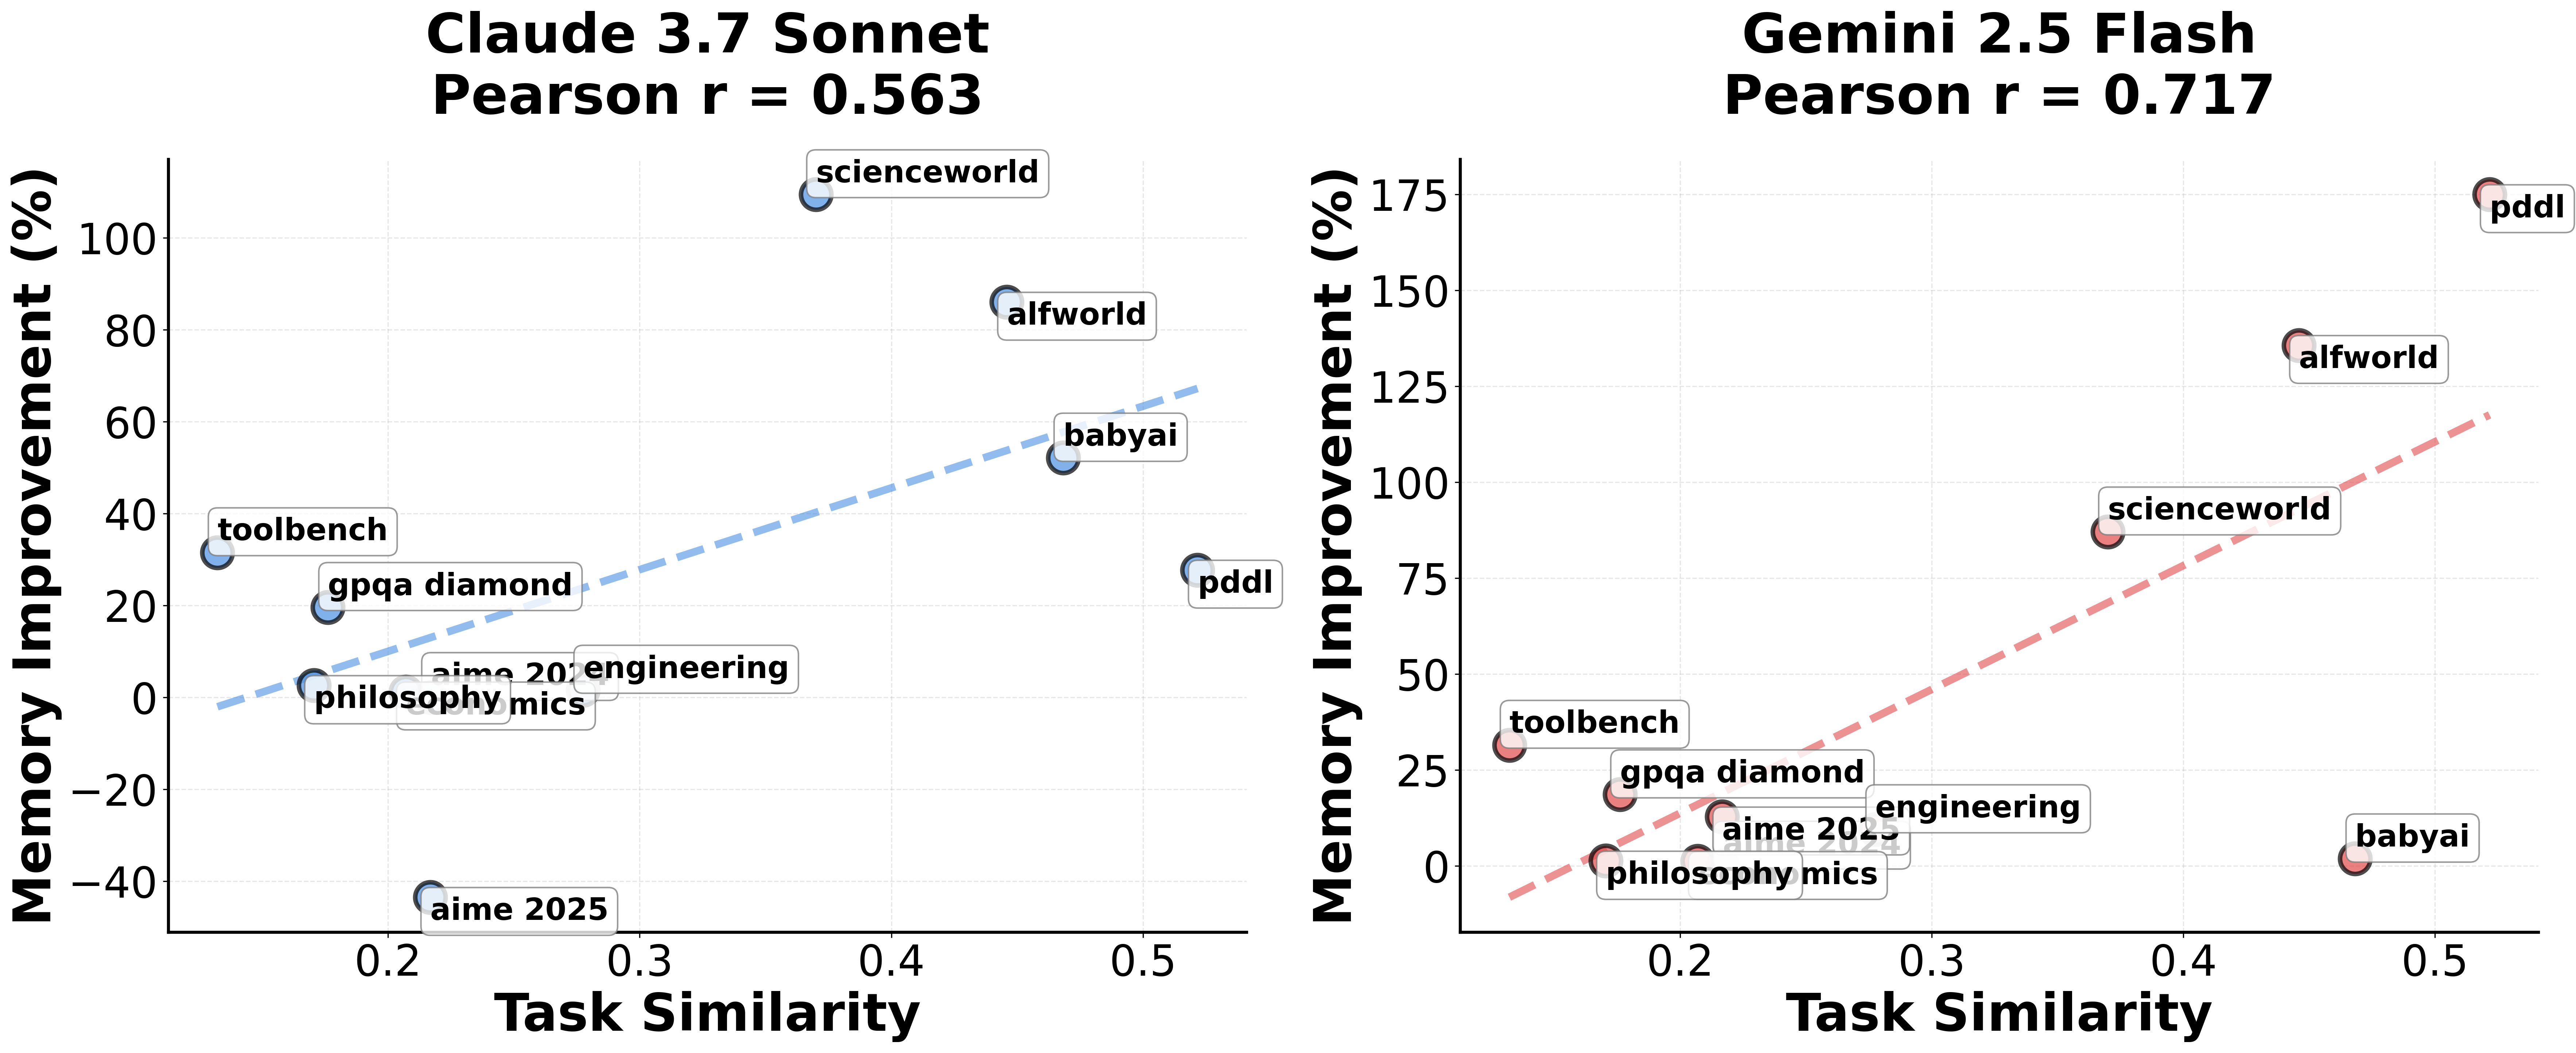
\includegraphics[width=\linewidth]{figures/correlation_side_by_side.png}
    \caption{ReMem performance gain over history baseline versus within-dataset task similarity.}
    \label{fig:correlate}
\end{figure}


\begin{figure}[t!]
    \centering
    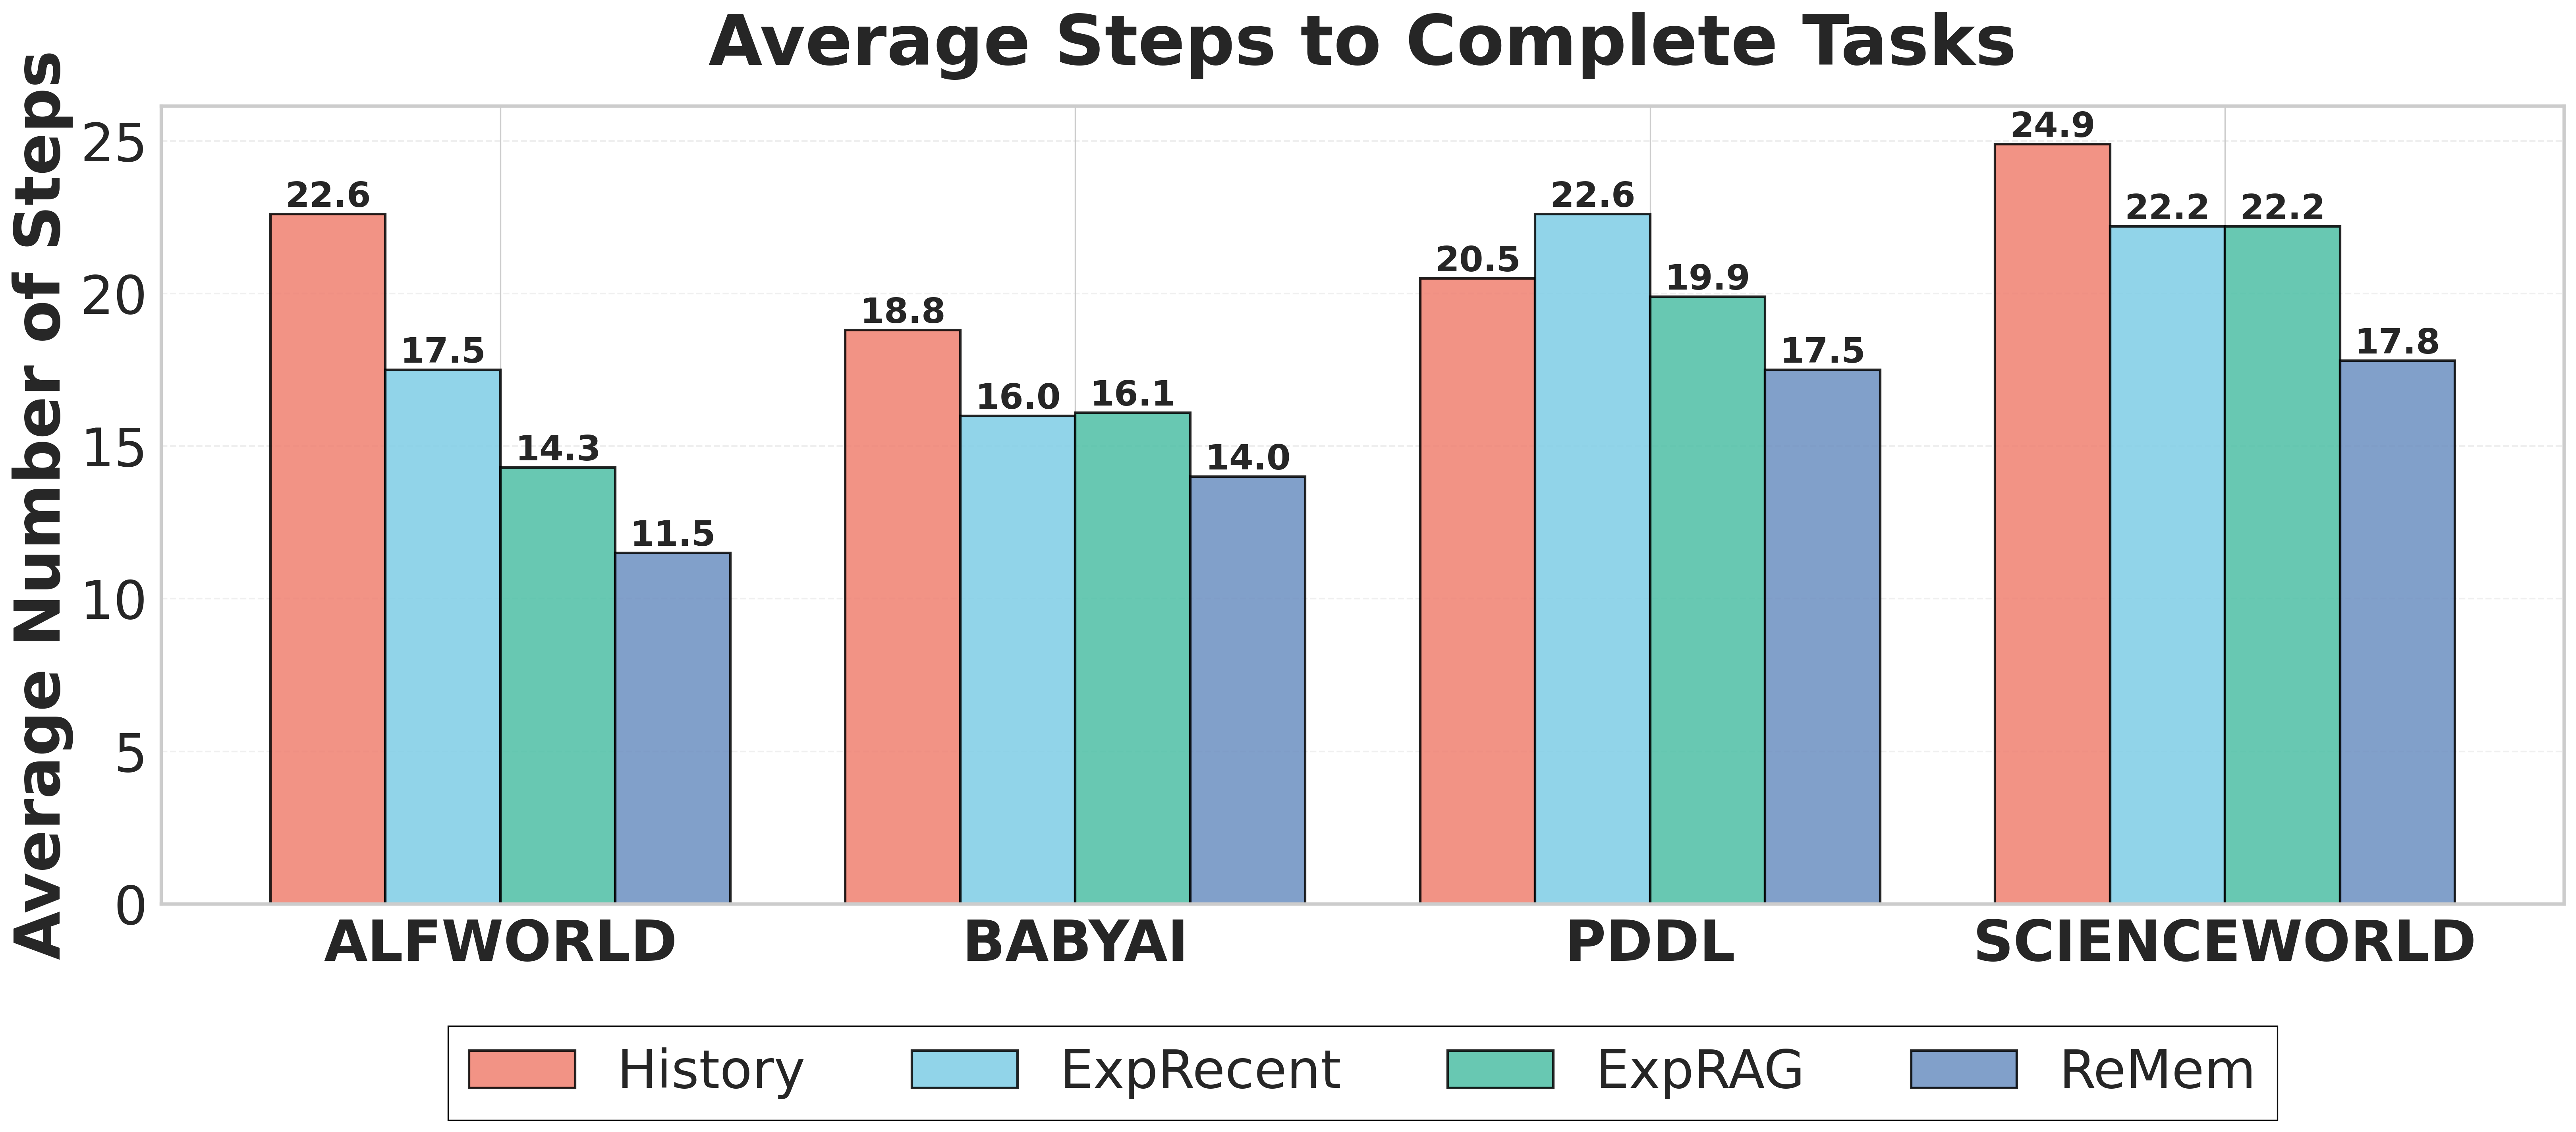
\includegraphics[width=0.85\linewidth]{figures/steps_comparison.png}
    \caption{Average steps to complete tasks across four benchmarks. We compare four methods: History, ExpRecent, ExpRAG, and ReMem. Lower is better. ReMem consistently requires fewer steps to complete tasks across all datasets, demonstrating more efficient task execution..}
    \label{fig:step}
\end{figure}




\subsection{Analysis of Memory Improvement (RQ2)}

Figure~\ref{fig:correlate} shows that \textsc{ReMem}'s improvement strongly correlates with within-dataset task similarity (Pearson $r=0.717$ on Gemini~2.5~Flash and $r=0.563$ on Claude~3.7~Sonnet).
Task similarity is measured by computing the average cosine distance between each task embedding and its dataset cluster center, where embeddings are obtained from the retriever encoder.
A smaller average distance indicates higher intra-dataset coherence and thus stronger structural similarity.
Tasks with higher embedding cluster ratios, such as PDDL and AlfWorld, yield larger gains, suggesting that recurring task structures facilitate memory reuse and generalization.
In contrast, more diverse or low-similarity datasets like AIME-25 or GPQA show smaller gains, reflecting limited transferable experiences.
These findings highlight the importance of embedding organization and semantic overlap in driving effective memory evolution. Further analysis of memory pruning rates can be found in Appendix~\ref{app:memory_prune}.

Figure~\ref{fig:step} compares step efficiency across four environments. 
Evolving-memory methods consistently require fewer steps to reach completion, with \textsc{ReMem} achieving the strongest and most stable reductions (e.g., from 22.6 to 11.5 steps on AlfWorld). 
The lightweight \textsc{ExpRAG} and \textsc{ExpRecent} also perform competitively, showing that simple task-level evolution can greatly improve efficiency without extra complexity. 
Overall, continual refinement not only boosts accuracy but also makes reasoning more focused and efficient.

\begin{table}[t!]
\centering
\small
\setlength{\tabcolsep}{4pt}
\renewcommand{\arraystretch}{1.2}
\scalebox{0.8}{
\begin{tabular}{llccccccc}
\toprule
\multirow{2}{*}{\textbf{Direction}} & \multirow{2}{*}{\textbf{Method}} 
& \multicolumn{2}{c}{\textbf{AlfWorld}} 
& \multicolumn{2}{c}{\textbf{ScienceWorld}} 
& \multicolumn{2}{c}{\textbf{Avg.}} \\
\cmidrule(lr){3-4} \cmidrule(lr){5-6} \cmidrule(lr){7-8}
 &  & S & P & S & P & S & P \\
\midrule
\multicolumn{2}{c}{Base} & 0.50 & 0.73 & 0.32 & 0.74 & 0.41 & 0.74 \\
\midrule
\multirow{3}{*}{Easy→Hard} 
 & ExpRecent & 0.66 & 0.82 & 0.48 & 0.83 & 0.57 & 0.83 \\
 & ExpRAG & 0.77 & 0.87 & 0.37 & 0.71 & 0.57 & 0.79 \\
 & ReMem & \textbf{0.91} & \textbf{0.96} & \textbf{0.63} & \textbf{0.88} & \textbf{0.77} & \textbf{0.92} \\
\midrule
\multirow{3}{*}{Hard→Easy} 
 & ExpRecent & 0.72 & 0.85 & 0.47 & 0.80 & 0.60 & 0.83 \\

 & ExpRAG & 0.87 & 0.92 & 0.51 & 0.81 & 0.69 & 0.87 \\
 & ReMem & \textbf{0.94} & \textbf{0.97} & \textbf{0.68} & \textbf{0.90} & \textbf{0.81} & \textbf{0.94} \\
\bottomrule
\end{tabular}}
\caption{Comparison of memory-based agents under different sequence difficulty directions. 
Each cell reports Success (S) and Progress (P). Easy→Hard and Hard→Easy indicate task order transitions, and averages (Avg) summarize per-direction performance.}
\label{tab:seq_difficulty}
\end{table}

\begin{table}[t!]
\centering
\small
\setlength{\tabcolsep}{6pt}
\renewcommand{\arraystretch}{1.15}
\scalebox{0.7}{
\begin{tabular}{l l cc cc cc}
\toprule
\textbf{Model} & \textbf{Method} & \multicolumn{2}{c}{\textbf{AlfWorld}} & \multicolumn{2}{c}{\textbf{ScienceWorld}} & \multicolumn{2}{c}{\textbf{Avg.}} \\
\cmidrule(lr){3-4}\cmidrule(lr){5-6}\cmidrule(lr){7-8}
 &  & S & P & S & P & S & P \\
\midrule
\multirow{9}{*}{Claude 3.7 Sonnet}
 & Amem        & 0.49 & 0.73 & 0.31 & 0.74 & 0.40 & 0.74 \\
\cmidrule(lr){2-8}
 & SelfRAG     & 0.47 & 0.73 & 0.34 & 0.73 & 0.41 & 0.73 \\
 & Mem0        & 0.49 & 0.73 & 0.36 & 0.74 & 0.43 & 0.74 \\
\cmidrule(lr){2-8}
 & DC-Cu       & 0.52 & 0.75 & 0.34 & 0.73 & 0.43 & 0.74 \\
 & DC-RS       & 0.51 & 0.74 & 0.38 & 0.74 & 0.45 & 0.74 \\
 & AWM         & 0.55 & 0.76 & 0.32 & 0.72 & 0.44 & 0.74 \\
\cmidrule(lr){2-8}
 & ExpRecent   & 0.62 & 0.80 & 0.34 & 0.74 & 0.48 & 0.77 \\
 & ExpRAG      & 0.76 & 0.90 & 0.27 & 0.63 & 0.52 & 0.77 \\
 & ReMem       & \textbf{0.92} & \textbf{0.96} & \textbf{0.69} & \textbf{0.91} & \textbf{0.81} & \textbf{0.94} \\
\midrule
\multirow{9}{*}{Gemini 2.5 Flash}
 & Amem        & 0.22 & 0.57 & 0.39 & 0.75 & 0.31 & 0.66 \\
\cmidrule(lr){2-8}
 & SelfRAG     & 0.25 & 0.58 & 0.36 & 0.71 & 0.31 & 0.65 \\
 & Mem0        & 0.25 & 0.59 & 0.34 & 0.71 & 0.30 & 0.65 \\
\cmidrule(lr){2-8}
 & DC-Cu       & 0.20 & 0.56 & 0.36 & 0.72 & 0.28 & 0.64 \\
 & DC-RS       & 0.21 & 0.57 & 0.36 & 0.71 & 0.29 & 0.64 \\
 & AWM         & 0.19 & 0.56 & 0.36 & 0.74 & 0.28 & 0.65 \\
\cmidrule(lr){2-8}
 & ExpRecent   & 0.22 & 0.57 & \textbf{0.59} & \textbf{0.86} & 0.41 & 0.72 \\
 & ExpRAG      & 0.25 & 0.60 & 0.51 & 0.78 & 0.38 & 0.69 \\
 & ReMem       & \textbf{0.57} & \textbf{0.76} & 0.50 & 0.75 & \textbf{0.54} & \textbf{0.76} \\
\bottomrule
\end{tabular}}
\caption{Results with both successful and failed task experiences on AlfWorld and ScienceWorld. Each cell reports Success (S) and Progress (P). Horizontal rules separate method families. Bold numbers denote the best results per metric within each model.}
\label{tab:multi_norm}
\end{table}





\subsection{Task Sequence: Easy v.s. Hard (RQ3)}

Table~\ref{tab:seq_difficulty} examines how memory-based agents adapt to changes in task difficulty.
Baseline methods exhibit noticeable degradation when moving from easier to harder tasks, revealing limited robustness under distribution shifts.
In contrast, evolving-memory agents, particularly \textsc{ReMem}, maintain strong and consistent performance across both directions, reaching up to 0.94/0.97 success and progress in the Hard$\rightarrow$Easy setting.
This stability shows that continual reflection enables \textsc{ReMem} to retain transferable knowledge even as task complexity varies.
The results further indicate that the design of task sequences, especially the ordering of difficulty levels, has a substantial impact on evaluating memory adaptation.
They also suggest that well-structured task progressions can actively facilitate learning by allowing models to build on prior experiences and generalize across increasingly complex challenges.
Together, these findings highlight the importance of standardized and thoughtfully organized task sequences for both fair evaluation and effective model development in future benchmarks.



\begin{figure}[t!]
    \centering
    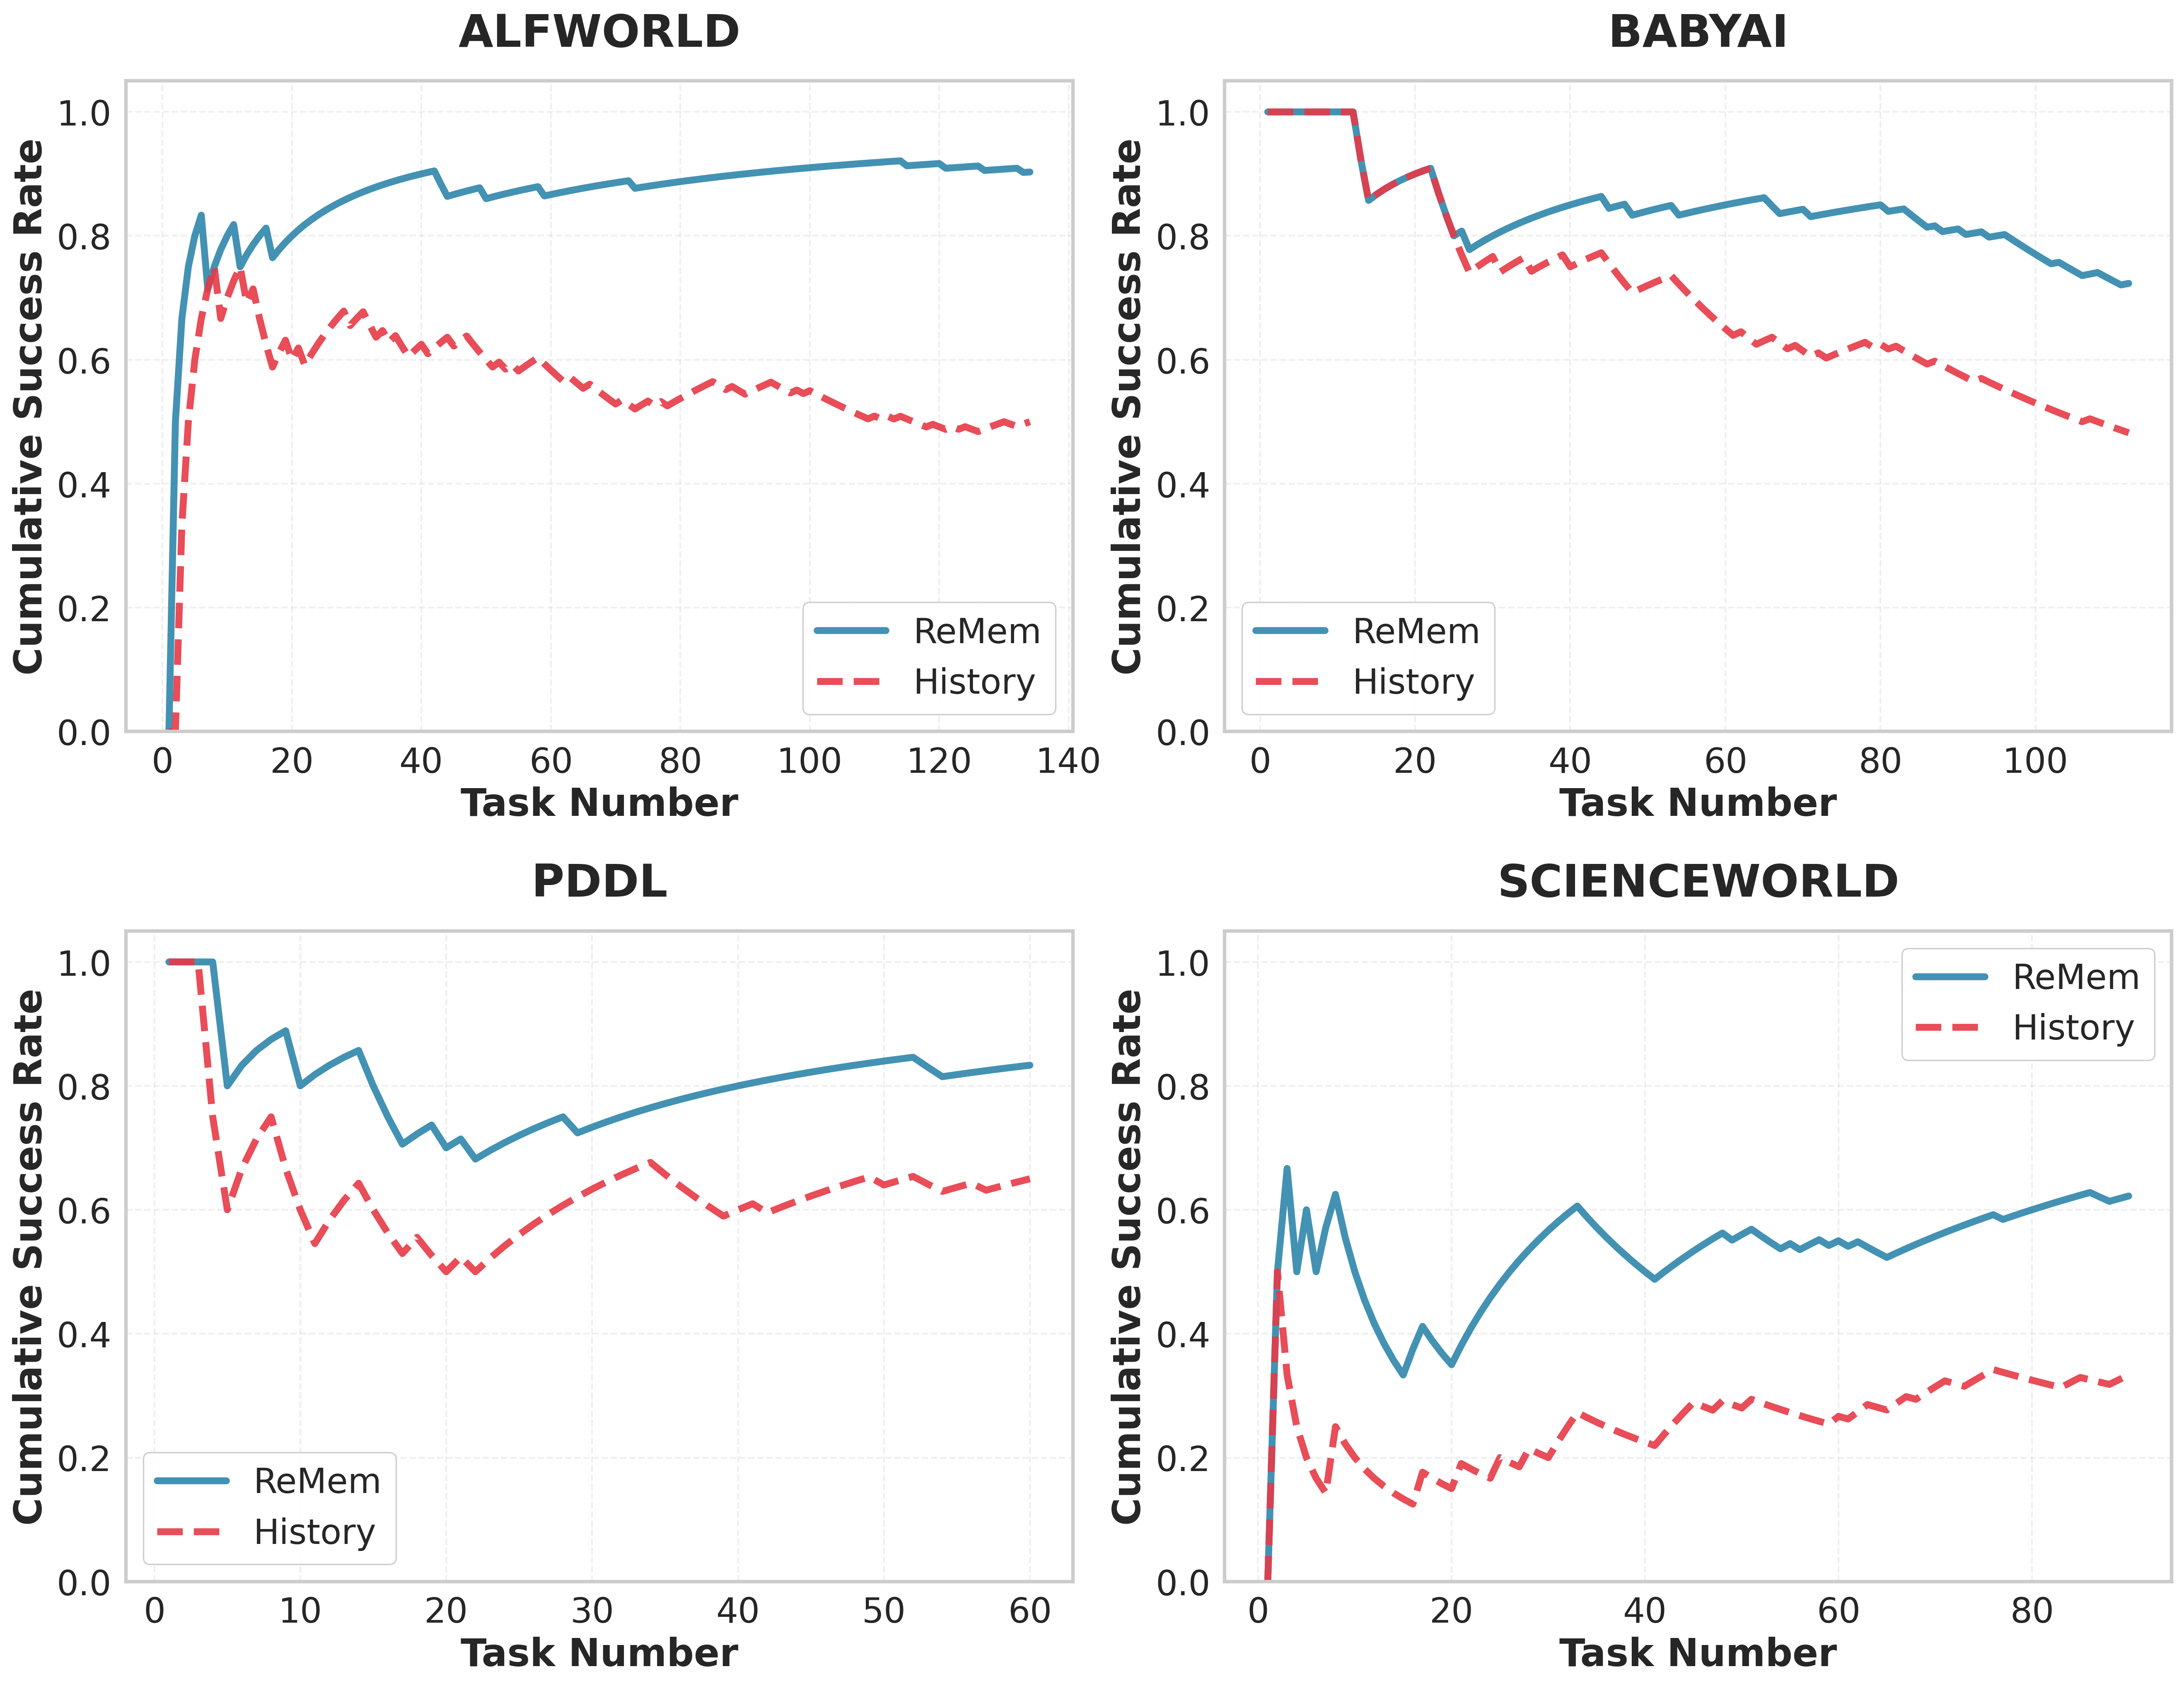
\includegraphics[width=0.8\linewidth]{figures/all_datasets_success_rate.png}
    \caption{Cumulative success rate across four interactive agent datasets. ReMem (solid blue) outperforms the History baseline (dashed red) on ALFWorld, BabyAI, PDDL, and ScienceWorld tasks. The rolling average shows performance trends as more task instances are evaluated.}
    \label{fig:curve}
    \vspace{-0.2cm}
\end{figure}



\subsection{Analysis of Feedback (RQ4)}
Table~\ref{tab:multi_norm} evaluates how agents perform when both successful and failed task experiences are stored in memory.
Baseline methods experience a clear performance drop when exposed to unfiltered failures, indicating that naive memory accumulation introduces noise and disrupts subsequent retrieval.
In contrast, evolving-memory approaches, particularly \textsc{ReMem}, remain robust by actively refining stored experiences, achieving the highest overall success and progress rates under both Claude and Gemini backbones.
These results demonstrate that selective utilization, which involves learning from successes while appropriately leveraging information from failures, is crucial for stable test-time adaptation.
They further highlight that memory refinement plays a central role in handling imperfect experiences and suggest that future work should explore failure-aware strategies for memory evolution.







\subsection{Performance w.r.t Time Steps (RQ5)}

Figure~\ref{fig:curve} shows the cumulative accuracy as tasks progress across four interactive environments.
The curves mainly serve to compare \textsc{ReMem} with the History baseline, as individual trajectories carry limited standalone meaning.
Across all environments, \textsc{ReMem} consistently achieves faster adaptation and more stable retention over time.
These results highlight that continual reflection enables \textsc{ReMem} to sustain performance across long task sequences, illustrating its robustness in test-time learning. More comparative results on single-turn tasks are presented in Appendix~\ref{app:curve}.















% \begin{figure}
%     \centering
%     \includegraphics[width=0.9\linewidth]{figures/rolling.pdf}
%     \caption{Rolling accuracy of the memory methods.}
%     \label{fig:placeholder}
% \end{figure}


